\documentclass[a4paper,11pt]{article} 
\usepackage[margin=1in]{geometry} 
\usepackage{amssymb}
\usepackage{amsmath,epsfig, epsf, epic, graphicx, fontenc} 
\usepackage{fancybox, lscape, subfigure} 
\usepackage{bm}
\usepackage{natbib}
%\usepackage{float}
\usepackage[margin=2cm]{caption}
\usepackage{setspace}
\usepackage{hyperref}
\usepackage{xcolor}

\allowdisplaybreaks

\usepackage{floatrow}

\title{Robust inference for geographic regression discontinuity designs: assessing the impact of police precincts}
\author{Emmett Kendall, Brenden Beck and Joseph Antonelli}
\date{}

\begin{document}

\maketitle

\begin{abstract}
We study variation in policing outcomes attributable to differential policing practices in New York City (NYC) using geographic regression discontinuity designs. By focusing on small geographic windows near police precinct boundaries we can estimate local average treatment effects of  precincts on arrest rates. The standard geographic regression discontinuity design relies on continuity assumptions of the potential outcome surface or a local randomization assumption within a window around the boundary. While these assumptions are often thought to be more realistic than other assumptions used to infer causality from observational data, they can easily be violated in realistic applications. We develop a novel and robust approach to testing whether there are differences in policing outcomes that are caused by differences in police precincts across NYC. In particular, our test is robust to violations of the assumptions traditionally made in geographic regression discontinuity designs and is valid under much weaker assumptions. We use a unique form of resampling to identify new geographic boundaries that are known to have no treatment effect, which provides a valid estimate of our estimator's null distribution even under violations of standard assumptions. We find that this procedure gives substantially different results in the analysis of NYC arrest rates than those that rely on standard assumptions, thereby providing more robust estimates of the nature of the effect of police precincts on arrest rates in NYC.  

    %Are there distinct differences in policing practices across precinct borders in New York City? Using applications of Geographic Regression Discontinuity Designs (GRDD), we seek to answer said question. We have incident level arrest and offense data from the New York City Police Department that provides spatial coordinates to each arrest in NYC since 2006. Using GRDD, we study the arrests that occur within a fixed-radius-boundary region of the border between two precincts. From here, we run an Auto Regressive Integrated Moving Average (ARIMA) test on the differences of arrests made by each precinct, scaled by the amount of crime in each precinct's specified boundary region. This will provide a novel p-value. In general, the distribution of p-values under the null hypothesis should follow a uniform distribution. However, this does not hold in our case, thus we need the null distribution of p-values. Using recursion, we can create new streets that ``match'' existing precinct borders and that are guaranteed to be under the null hypothesis. Running the ARIMA procedure at each ``match'' we can get a null distribution for the p-value for each precinct border on the map. Then, treating the initial p-value as a test statistic, we can see if it is in fact significant. While the data analysis is not quite finished yet, initial tests indicate that our methodology is sound. Although initial data analysis shows failure in certain causal assumptions, we have developed a design that will allow for valid inference.
\end{abstract}

\section{Introduction}

Policing varies across political boundaries, such as state or city borders. Such differences are expected, but we know very little about whether smaller, sub-municipal boundaries like police districts, precincts, and service areas also influence police outcomes \citep{klinger1997negotiating}. This lack of research persists despite police officers reporting that their behavior and perception is influenced by precinct boundaries \citep{hassell2007variation}. Understanding whether precincts police differently has important implications for equity and policy. Variation in policing between cities is tolerated because it results, in part, from the electoral choices of residents. Variation within cities, however, generates a more troubling kind of inequality. Residents do not vote for their police precinct commander and they expect treatment equal to that of people in other neighborhoods. Policing variation generated by precinct differences might also compound other forms of spatial inequity like residential segregation, racial bias, or high crime areas \citep{bell2020anti}. 

Another potential consequence of between-precinct variation in policing is diminished policy efficacy. Some recent police reform efforts have included attempts to reduce the number of pedestrian stops and frisks, reduce police officers' use of deadly force, and improve police-community relations. Most reforms to achieve these goals are implemented at the city scale, but if significant variation exists between precincts, such a one-size-fits-all approach might fail. Even place-based interventions like hot-spots policing target high-crime areas and ignore precinct boundaries. Crime research has long understood the salience of micro places in shaping crime, but policing research is only recently catching up to how local characteristics shape policing. It is likely that police behavior, like criminal behavior, varies greatly by place. In this study, we examine the 77 precincts of the New York City Police Department (NYPD) to estimate whether police precincts causally affect arrest rates.

This is a difficult question to answer because the regions each police precinct covers are different from one other with respect to important demographic and criminological variables. One precinct might have different low-level arrest rates than another because it has higher crime rates, more targets for theft, or more transient populations. Therefore, we have to isolate the effect of the police precincts themselves. Randomization is the gold standard for drawing causal conclusions, but while these are occasionally available in the criminology literature to evaluate policies like hot spots policing \citep{puelz2019graph}, in many scenarios they are not available or feasible. When evaluating the impact of police precincts, we can not randomize individuals to a police precinct by forcing them to live or work in certain areas of a city. The ubiquity of observational studies has led to a wide range of approaches to estimate causal effects under as weak of assumptions as possible. Common approaches are difference-in-difference estimators \citep{ashenfelter1984using, lechner2011estimation}, the regression discontinuity design \citep{thistlethwaite1960regression,imbens2008regression, cattaneo2019regression}, interrupted time series analysis \citep{cook1979quasi, bernal2017interrupted}, and synthetic control analysis \citep{abadie2010synthetic}, among others. In the context of policing and criminology, these ideas have been used to address important issues, such as whether increased oversight of police leads to increases in crime and decreased effectiveness of the police force \citep{ba2019effect}, quantifying the impact of a penalty system for drivers in Italy on traffic incidents and traffic-related fatalities \citep{de2013deterrent}, or estimating the heterogeneous effects of neighborhood policing \citep{antonelli2020estimating, beck2020effects}.

In this study we focus on the regression discontinuity design and its extensions to geographic settings. For an in-depth review of regression discontinuity designs and implementation details, see \cite{imbens2008regression} and \cite{cattaneo2019regression}. The traditional regression discontinuity design occurs when treatment assignment is either partially or completely determined by a pre-treatment covariate, typically referred to as the running or score variable. There exists a cutoff value of this running variable, above which units receive treatment, and below which units receive the control. The fundamental idea is that units within a small distance around the cutoff value form a locally randomized experiment \citep{mattei2017regression}. The estimand of interest is a local treatment effect near the cutoff value, and nearby observations are used to extrapolate what would happen both under treatment and control at this boundary value. This approach has been extended to multivariate running variables such as the results of two types of educational tests \citep{matsudaira2008mandatory}. A specific example of a bivariate running variable is found in the geographic regression discontinuity design where latitude and longitude are used to determine treatment assignment. Important aspects specific to the geographic design are highlighted in \cite{keele2015geographic}. This design has been used to estimate the effect of private police departments on crime \citep{macdonald2016effect}, the impact of voter initiatives on voter turnout \citep{keele2015enhancing}, the effect of the Civil Rights Act of 1875 \citep{harvey2020applying}, and whether school districts impact housing prices \citep{rischard2020school}. 

Regression discontinuity designs rely on assumptions that state that the potential outcomes are smooth at the cutoff value or that treatment behaves as if it were randomized within a window around the cutoff value. To assess the validity of these assumptions, a number of falsification tests have been proposed. A negative control approach is to treat an observed covariate as an outcome, where we know the treatment should not affect this covariate and estimate the treatment effect on this covariate to see if the approach correctly estimates a null association \citep{lee2004voters}. Another issue is that the running variable can be manipulated by subjects if they are aware of the cutoff value, and this can be evaluated by checking if the running variable is continuous at the cutoff \citep{mccrary2008manipulation, cattaneo2017comparing}. Other approaches examine the sensitivity of results to bandwidth selection \citep{lemieux2008incentive}, as robustness of results to this choice provides increased belief in the resulting findings. 

While these approaches can potentially highlight issues with the assumptions inherent to the regression discontinuity design, they do not correct for violations of these assumptions. In this work, we provide valid inference of the effect of police precincts on arrest rates in New York City. By using a novel resampling scheme, our approach allows for violations of the assumption that treatment is as randomized within a window around the cutoff point of the running variable. We exploit a large spatio-temporal data set of crime and arrest data in NYC to find streets that behave similarly to precinct boundaries, but by definition have no precinct effect as they are fully contained within a single police precinct. We use these streets to construct a null distribution that accounts for violations of local randomization assumptions and provides a valid hypothesis test of individual precinct effects as well as an estimate of the overall degree of variation in policing. 

\section{Policing data in NYC and preliminary analyses}
\label{sec:data}
Our analyses draw on two data sources made public  by the NYC police department (NYPD): NYPD Arrest Data and NYPD Complaint Data. Both provide information at the incident level with geolocated, address data for all arrests and all crimes reported to the police in the years 2010-2018. The NYPD is divided into 77 police precincts, each patrolling a particular geographic area of the city. We exclude the precinct corresponding to Central Park, which does not have any residents, leading to 76 precincts in total.  Covariate information is available at a less spatially resolved level, as we have census-tract level covariate information provided by the United States Census Bureau's American Community Survey. Our goal is to use this data to understand whether there is variability in the arresting practices across precincts in New York City, and whether individuals are more or less likely to be arrested depending on which precinct's police force they are exposed to.

Using this data, we can visualize both when and where arrests occur as well as the precinct from which the arresting officer originates. Figure \ref{fig:Precinct77} highlights the arrest data for Precinct 77 in NYC during the year 2014, both with and without the roadmap of the city overlaid on the figure using the R package \texttt{ggmap}  \citep{ggmap2013}. 
\begin{figure}[h]
    \centering
    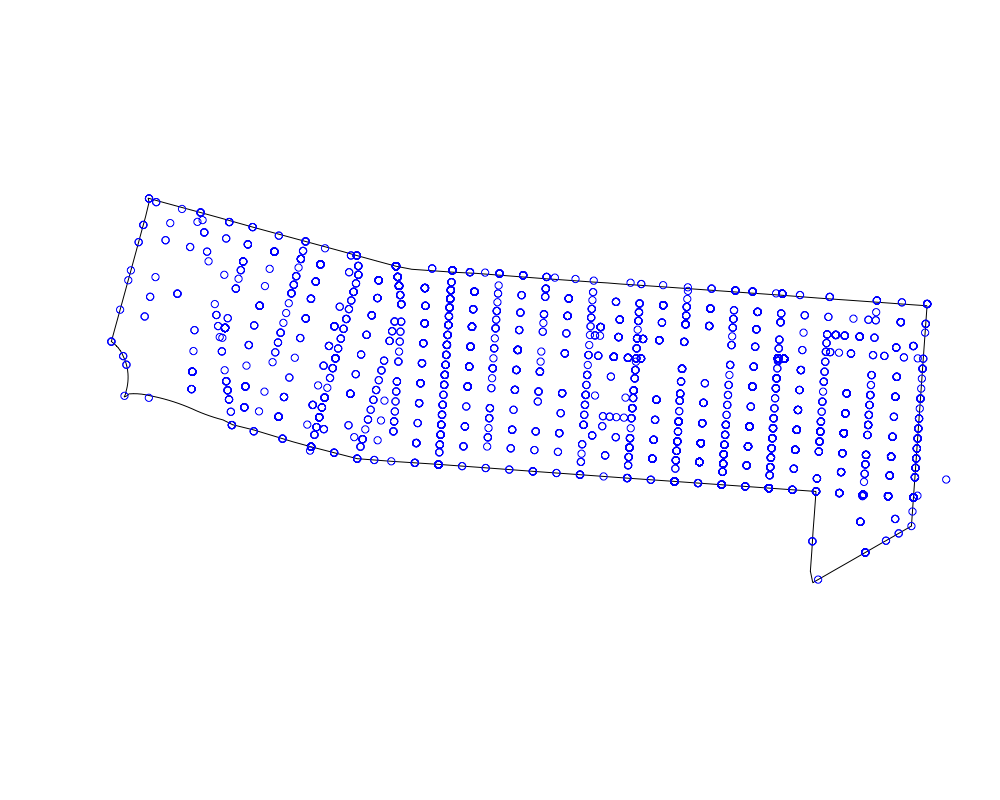
\includegraphics[scale=0.2]{plots/ArrestsPrec77.png} 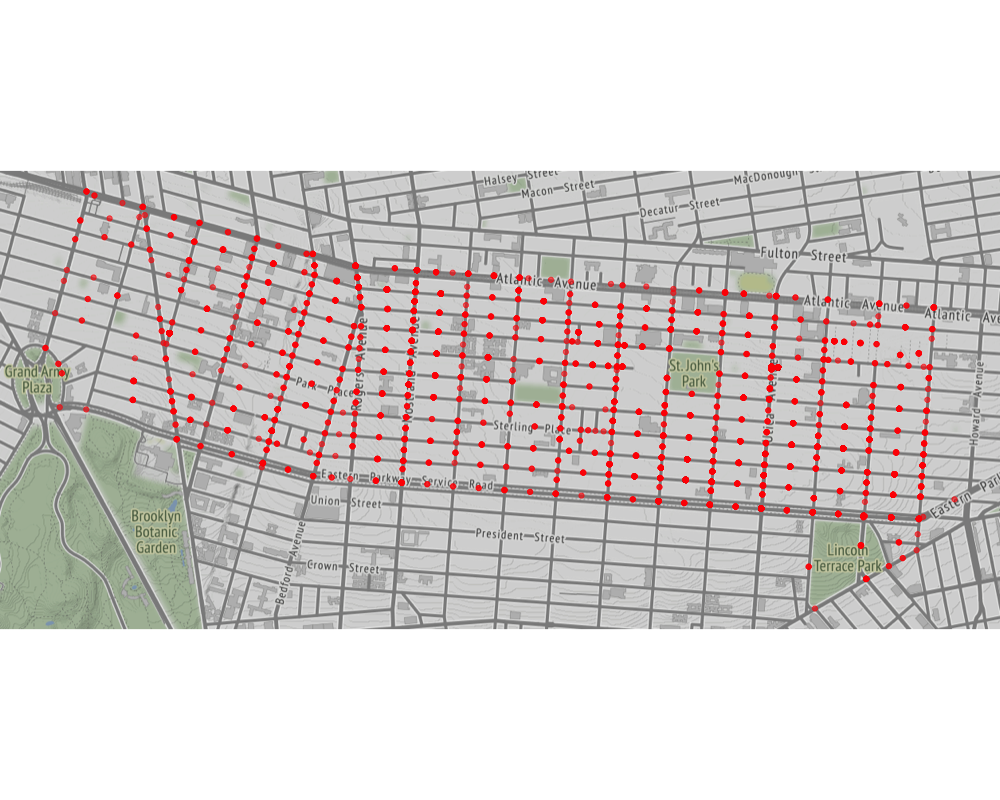
\includegraphics[scale=0.2]{plots/ArrestPrec77GoogleMaps.png}
    \caption{Arrest locations from officers of precinct 77 in NYC during the year 2014.}
    \label{fig:Precinct77}
\end{figure}
This figure reveals features of the data we will leverage in our approach to inference. The arrests fall directly on streets themselves, and are not spread out across the entire spatial domain. This is because arrests are recorded at addresses, and addresses are restricted to streets, regardless of where within a property arrests occur. Additionally, precinct boundaries are streets themselves, and there are arrests that fall directly on this boundary. 

Suppose for now that we are interested in estimating whether there is a difference in arresting practices between two neighboring precincts. Formally, we want to assess whether there is a causal effect of police precinct on arrest rates. Given the lack of rich covariate information, but high degree of spatial resolution, one might choose to use a geographic regression discontinuity design (GeoRDD) to estimate the effect of police precincts between two nearby regions. The GeoRDD leverages the fact that nearby observations should be similar with respect to important unobserved characteristics that are associated with arrest rates. In this context, this assumption would be satisfied if areas on either side of the border between the two precincts are similar to each other. Individuals do not choose where they live based on police precincts, and most do not even know which precinct they live in. Therefore any differences we see in arrest rates would be attributable to differences in police precinct practices. We can draw a buffer zone around the border of two precincts and study the difference in arrest rates made by each precinct in the buffer over time. An illustration of the setup can be found in Figure \ref{fig:Precinct77_79} \textcolor{red}{(redraw these images with rounded borders)}, where arrests are color coded such that blue dots correspond to arrests made by precinct 83 on the left and precinct 14 on the right, and red dots are arrests made by precinct 81 on the left and precinct 10 on the right. 
% \begin{figure}
%     \centering
%     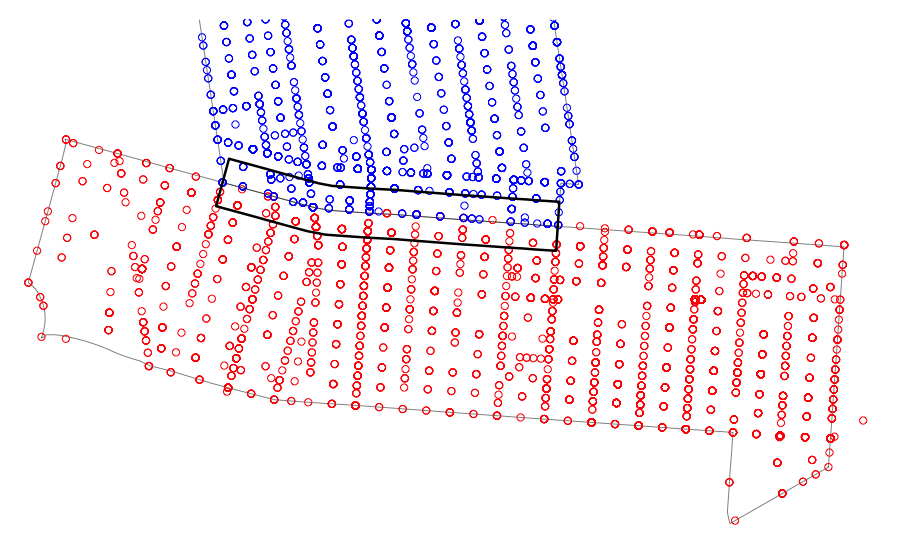
\includegraphics[scale=0.25]{plots/Prec77and79Buff.png}
%         \caption{Arrest locations for precinct 77 (green) and precinct 79 (blue) during the time frame XX-YY}
%     \label{fig:Precinct77_79}
% \end{figure}
\begin{figure}[h]
    \centering
    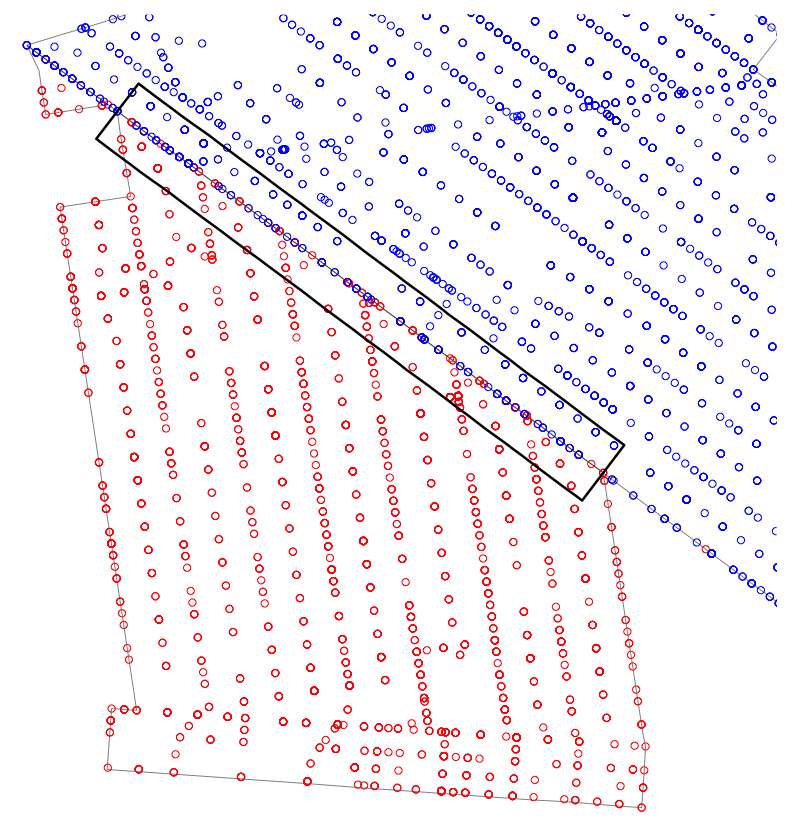
\includegraphics[scale=0.20]{plots/Buff81and83.png}
    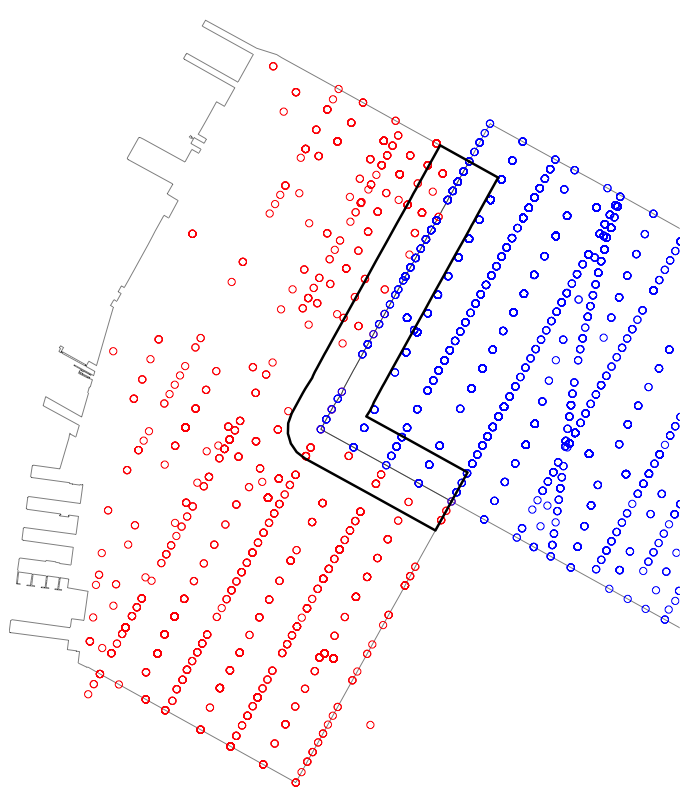
\includegraphics[scale=0.20]{plots/Buff10and14.png}
        \caption{Arrest locations for precinct 81 and 83 (left) and for precincts 10 and 14 (right)}
    \label{fig:Precinct77_79}
\end{figure}
We see that for some borders, all arrests on the border itself are made by one precinct, while on other borders the arrests on the border are randomly distributed between the two precincts. For this reason, we use an updated buffer zone that includes all arrests within a particular distance, excluding those arrests made on the border. This should remove any biases induced by strange behavior at the border, but still be comparing two similar regions. 
If there is no variation in policing practices across precincts, and under certain causal assumptions that we detail in the following section, we would expect each null hypothesis of no precinct effect at every precinct border to be rejected with probability $\alpha$, where $\alpha$ is our pre-specified type I error. Given that there are 158 borders, we would expect to see roughly $\alpha \times 158$ significant associations and the distribution of p-values across these tests to be roughly uniformly distributed if police precincts do not affect arrest rates. 

% Include these results to illustrate that this naive thing is pervasive
Suppose a novel binomial test is performed at each of the 158 borders for different window lengths. Buffers with window lengths 200 ft, 300 ft, ..., 800 ft are drawn around each border. Then, we count the arrests made by each of the two precincts within the bounds of the buffer zone and test if there is a difference in the counts of arrests. As mentioned before, if there exists no precinct affect, we should expect that the counts of arrests on either side of the border to be relatively similar and therefore, by chance, we see a significant difference in arrests in $\alpha \times 158$ borders. Under the assumption of ``no precinct effect,'' we know that the histogram of p-values obtained from the 158 separate binomial test should also be relatively uniform. \textcolor{red}{(remake these pictures)} However, Figure \ref{fig:NaivePvalue} shows the distribution of p-values when using a buffer width of 500 feet, and the percentage of rejections out of 158 borders that are obtained as a function of the buffer width. We see that 65.3\% of the p-values are less than 0.05 when we use a buffer width of 500 ft, with similar percentages for other buffer widths.
\begin{figure}[h]
    \centering
    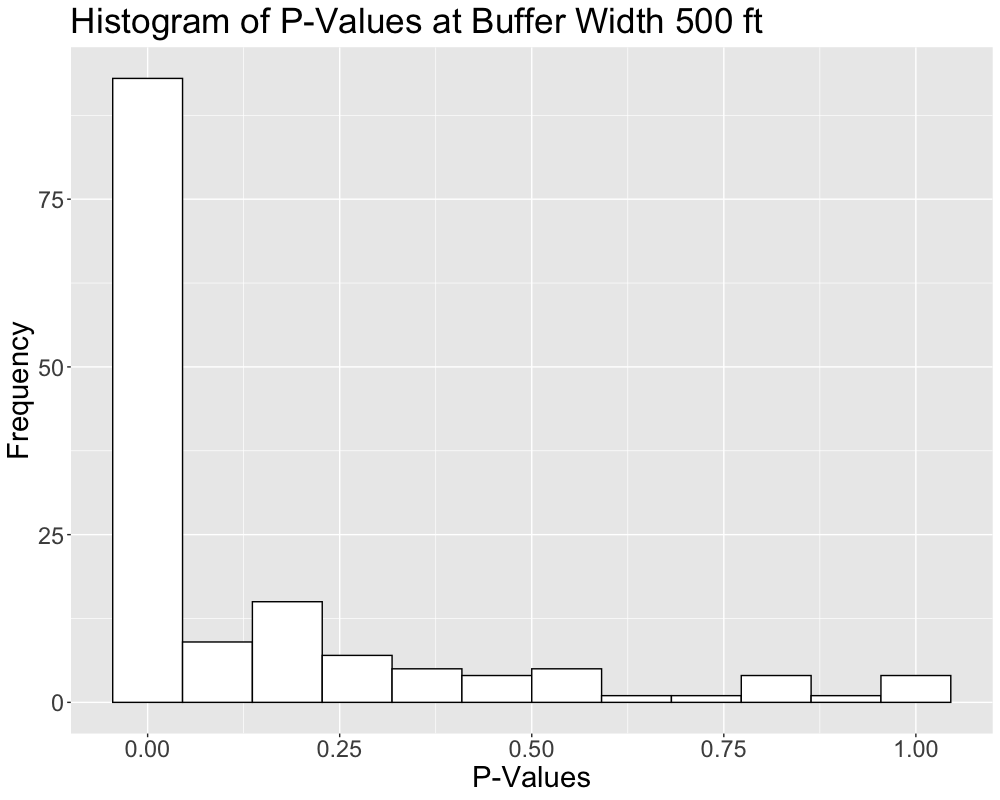
\includegraphics[scale=0.2]{plots/UnadjPVal500.png}
    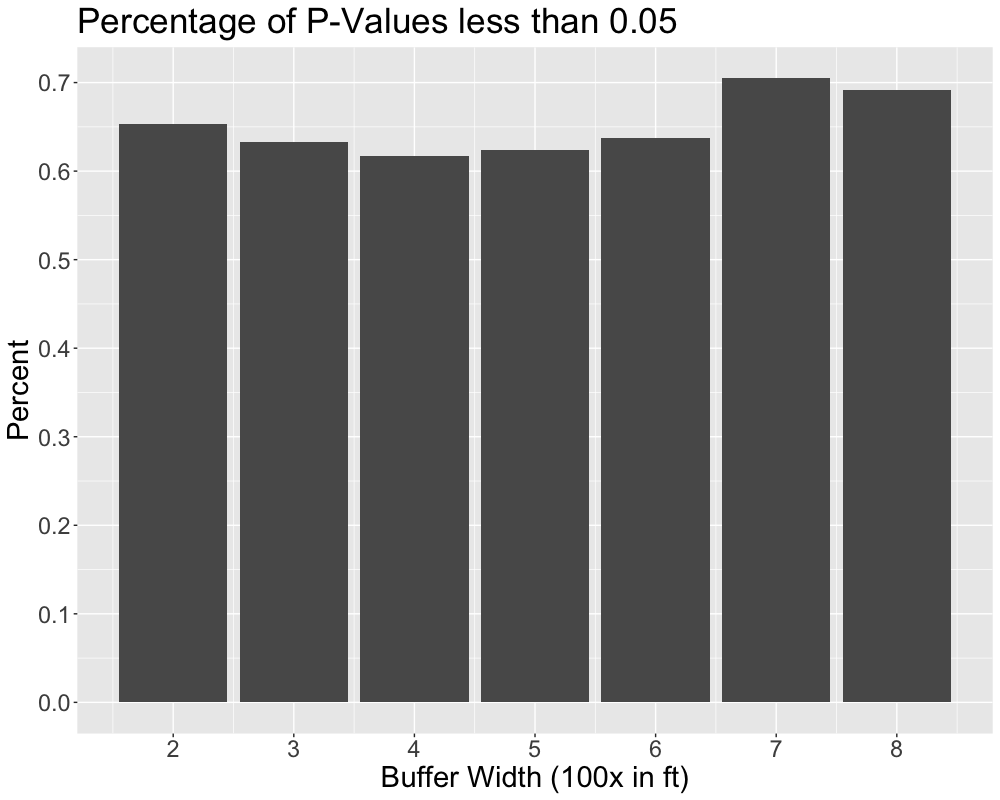
\includegraphics[scale=0.2]{plots/NumRejectByBuffer.png}
        \caption{Distribution of p-values across all 158 borders at buffer of 500 feet (left) along with the percent of rejections as a function of window size around the border (right).}
    \label{fig:NaivePvalue}
\end{figure}
There are a number of reasons why this might occur: 1) there truly are vast differences in arresting practices spread across NYC, 2) either the causal assumptions do not hold or the statistical test we use is invalid, or 3) some combination of these two issues.

\subsection{Negative Control (trees in NYC) (emmett)}
With the heavily skewed p-value distribution, it sparks curiosity into learning more about the structure of these data. In particular, is the fact that arrest locations are only spatially labelled on streets affecting these p-values for the novel binomial test? Therefore, take the 2015 Street Tree Census data set provided by \textit{NYC Open Data}. Shown below \textcolor{red}{(include similar plot of tree locations)} are the locations of trees throughout NYC. We would expect that the difference in tree populations between two bordering precincts to be miniscule. In other words, after performing the same binomial test with the Tree Census data, we should not expect to see a significant difference in tree counts on either side of a precinct border within the different buffers. However, below, we show the same figures as what we got for the arrest data \textcolor{red}{(include figures of naive binomial test for neg control)}. The same skewed trends exist on a data set where we know that there should not exist a difference across a precinct boundary. 

Hence, based on the analysis as it stands, we cannot differentiate between a conclusion that precincts truly affect arrest rates or invalidity of our statistical analyses. Thus, we seek to develop a methodology that relies on weaker assumptions than traditional geographic regression discontinuity designs, and therefore provides more reliable inference on the effect of police precincts. 

\section{Methodology section}

The observed data on our outcome of interest consists of a set of times and geographic locations corresponding to each arrest in New York City between 2010 and 2018. Our data can be thought of as generated from a point process, in that an arrest will randomly occur at some time point, and at a given location. We denote geographical coordinates by $\boldsymbol{S} = (S_{1}, S_{2})$, which correspond to latitude and longitude. Since we are interested in studying variability in arrest rates across space, rather than time, we aggregate across the temporal component and convert our data to monthly-level. Therefore our observed outcomes are given by $\mathcal{S}_t = \{\boldsymbol{S}_{t1}, \boldsymbol{S}_{t2}, \dots, \boldsymbol{S}_{t N_t}\}$ for $t=1, \dots, T$. Here, $\boldsymbol{S}_{t1}, \boldsymbol{S}_{t2}, \dots, \boldsymbol{S}_{t N_t}$ represent the locations at which an outcome is observed during time period $t$. We use $|\mathcal{S}_t| = N_t$ to denote the cardinality of this set, which corresponds to the number of events in the entire study domain during time period $t$. 

Our focus will be on specific subregions of the entire spatial domain and therefore we can define corresponding region specific quantities. Let $R$ be a part of the geography under study, such as the area within 200 feet of a precinct boundary. We let $Y_t(R) = \sum_{i} I(\boldsymbol{S}_{ti} \in R)$ represent the number of outcomes that occurred in region $R$ at time $t$. We assume that our data follow an inhomogeneous point process \citep{daley2003introduction} with intensity function given by $\lambda(\boldsymbol{s})$. Specifically, this implies that $$E(Y_t(R)) = \Lambda(R) = \int_R \lambda(\boldsymbol{s}) d \boldsymbol{s}.$$
Additionally, this implies that if $R_1, R_2,..., R_K$ are $K$ non-overlapping regions of the domain of interest, then $(Y_t(R_1), Y_t(R_2), \dots, Y_t(R_K))$ are independent random variables with expected values given by $(\Lambda(R_1), \Lambda(R_2), \dots, \Lambda(R_K)).$ Note that for now, we are letting the intensity function be time-invariant, though this can be extended to allow for time-specific intensity functions $\lambda(\boldsymbol{S}, t)$. 

\subsection{Single border estimands}

Now that we have introduced notation for point process data, we can formally define potential outcomes and estimands of interest. Our interest is in whether or not police precincts play a role in arresting rates throughout NYC, but we first focus on two adjacent precincts, which we refer to as precinct A and precinct B. We extend these ideas to all adjacent precinct pairs in NYC in Section \ref{sec:Global}. We define our treatment variable $T(\boldsymbol{S})$ to be an indicator of whether a location is policed by police precinct A or B. Clearly, this is a deterministic function of $\boldsymbol{S}$ as $T(\boldsymbol{S}) = I(\boldsymbol{S} \in R_A)$ where $R_A$ is the region that defines precinct A. This is referred to as a sharp regression discontinuity design as the forcing variable $(\boldsymbol{S}$ in this setting) completely determines the treatment assignment \citep{trochim1990regression}. 

We frame our problem and the regression discontinuity design that we use within the potential outcomes framework \citep{rubin1974estimating}. We define $\mathcal{S}_t^1$ to be the set of outcomes with an arrest had every location been exposed to policing by precinct A and $\mathcal{S}_t^0$ be the corresponding quantity for precinct B. Accordingly, we can define $Y_t^1(R)$ to be the number of outcomes we would observe in region $R$ if exposed to policing by precinct A and $Y_t^0(R)$ be the same quantity for precinct B. We assume that these potential outcome point patterns come from inhomogeneous point processes with intensity functions $\lambda^1(\boldsymbol{s})$ and $\lambda^0(\boldsymbol{s})$, respectively. Precincts A and B could have different arrest rates for a number of reasons, many of which are not due to differential policing by the respective police precincts. One area could have higher crime rates, different types of crimes committed with different clearance rates, or a different demographic of individuals in the population that live there. For this reason, we will focus on the boundary between the two precincts, as the individuals on either side of the boundary are more likely to be similar and crime characteristics should be more comparable. We denote all points on the boundary of the two precincts by $\mathcal{B}$. Further, define a distance function $d(\boldsymbol{s}, \mathcal{B})$, which is the shortest distance between $\boldsymbol{s}$ and the boundary. We focus on a local average treatment effect defined by 
\begin{align}
  \theta_{\delta} = E(Y_t^1(R_{\delta}) - Y_t^0(R_{\delta})) = \int_{R_{\delta}} \{ \lambda^1(\boldsymbol{s}) - \lambda^0(\boldsymbol{s}) \} d \boldsymbol{s},  \label{eqn:LATE}
\end{align}
where $R_{\delta} = \{ \boldsymbol{s}:d(\boldsymbol{s}, \mathcal{B}) < \delta \}$. Intuitively $R_{\delta}$ is the region within distance $\delta$ of the boundary between precinct A and precinct B. Similar ideas could be used to target other estimands. One such estimand, which acknowledges the fact that the treatment effect might differ on different parts of the boundary can be defined as 
$$\tau(\boldsymbol{b}) = \lambda^1(\boldsymbol{b}) - \lambda^0(\boldsymbol{b}),$$
which is a point process extension to the estimands seen in previous spatial regression discontinuity designs \citep{keele2015geographic, rischard2020school}.

\subsection{Identifying assumptions and potential for bias}

The main idea behind the regression discontinuity design is that by looking in a close window around the boundary, the two regions on either side of the boundary are very similar with respect to all important features except for which precinct they are being policed by. We can therefore compare outcomes on either side of the boundary and attribute differences to the effect of the police precincts. Here we formalize this notion by explicitly writing down the assumptions by which the regression discontinuity design is able to identify the local average treatment effect in this setting. First, define $R_{\delta, 1} = \{ \boldsymbol{s}:d(\boldsymbol{s}, \mathcal{B}) < \delta, T(\boldsymbol{s}) = 1 \}$ and $R_{\delta, 0} = \{ \boldsymbol{s}:d(\boldsymbol{s}, \mathcal{B}) < \delta, T(\boldsymbol{s}) = 0 \}$ to be the regions of $R_{\delta}$ that correspond to precincts A and B, respectively. We are now in a position to state the assumptions under which the local average treatment effect can be identified from the observed data. \\
\\
\textbf{Assumption 1:} \textit{Constant integrated intensity functions}. $$\Lambda^1(R_{\delta, 1}) = \Lambda^1(R_{\delta, 0}), \quad \Lambda^0(R_{\delta, 1}) = \Lambda^0(R_{\delta, 0})$$
\textbf{Assumption 2:} \textit{Consistency of potential outcomes}. $$Y_t^T(R_{\delta, T}) = Y_t(R_{\delta, T})$$
The first assumption states that for both the control and treated potential outcome point processes, the expected number of events that fall on one side of the boundary within a distance of $\delta$ is the same regardless of which side of the boundary is being looked at. This is similar to local randomization assumptions typically made in regression discontinuity designs. This assumption is needed because we need to use what happened under the precinct A side of the border to infer what would happen on the precinct B side of the border had they been exposed to policing by precinct A. Assumption 2 is required to link our observed data to the potential outcomes. Given both of these assumptions, we can identify the effect of interest as
\begin{align*}
    E(Y_t^1(R_{\delta})) &= E(Y_t^1(R_{\delta, 1})) + E(Y_t^1(R_{\delta, 0})) \\
    &= \Lambda^1(R_{\delta, 1}) + \Lambda^1(R_{\delta, 0}) \\
    &= 2 \Lambda^1(R_{\delta, 1}) \\
    &= 2 E(Y_t(R_{\delta, 1})),
\end{align*}
which is a fully observable quantity. An analogous identification strategy could be used to identify $E(Y_t^0(R_{\delta}))$. Assumption 1 and the identification strategy here can be extended to condition on covariates, however, we do not discuss this throughout for simplicity and because we do not have covariates that are spatially or temporally resolved enough to use in our study. 

The biggest concern when using the regression discontinuity design is that the aforementioned assumptions do not hold. While assumption 2 is reasonable and likely to hold in most applications, assumption 1 is relatively strong and can fail in many scenarios. This is problematic because a violation of assumption 1 can lead to bias in the estimated treatment effects and inflation of type I error rates. In the New York City example, this assumption would be violated if the communities on either side of the boundary are systematically different with respect to the outcome of interest. While we can limit this by forcing $\delta$ to be as small as possible, neighborhoods in New York City can change drastically even by moving just one block. Our interest will be in testing the null hypothesis $H_0: \theta_{\delta} = 0$, and our goal will be to create a hypothesis test that has valid type I error, even in the presence of violations of assumption 1. 

\subsection{Resampling to obtain robust test of null treatment effect}

To test $H_0: \theta_{\delta} = 0$, we perform a two step procedure. The first step is to come up with a test statistic and associated p-value for testing this null hypothesis. The second involves resampling new boundaries in New York City to estimate the distribution of this statistic under the null hypothesis of no precinct effect. For step one, we can define $$Z_t = Y_t(R_{\delta, 1}) - Y_t(R_{\delta, 0}),$$ which is the difference in the number of arrests in $R_{\delta, 1}$ and $R_{\delta, 0}$. If $Z_t$ is positive and large on average, this indicates that precinct A arrests more individuals than precinct B. We then fit the following autoregressive model of order $Q$ to $Z_t$:
\begin{align}
    Z_t = c + \sum_{q=1}^Q \rho_q Z_{t-q} + \epsilon_t. \label{eqn:TestStatistic}
\end{align}
To test whether one precinct has higher arrest rates than the other, we will test $H_0: c = 0$ versus $H_a: c \neq 0$. The key feature is that under assumptions 1 and 2, testing $c = 0$ corresponds to testing whether $\theta_{\delta} = 0$. Therefore, if we perform a valid test of whether $c=0$, we have a valid test of whether the treatment effect is zero. For obtaining statistical validity, we need to understand the distribution of $\widehat{c}$ under the null hypothesis. Typically, inference proceeds by assuming that $\widehat{c} / \widehat{\sigma}_c$ follows a standard normal distribution, where $\widehat{\sigma}_c$ is an estimate of the standard error of $\widehat{c}$. Unfortunately, this can fail for a number of reasons. Even if assumptions 1 and 2 hold, this distributional result on the test statistic may fail due to small sample sizes, model misspecification, or not properly accounting for temporal correlation in the data. Of even greater concern is that assumption 1 does not hold. If assumption 1 is violated, nearby regions on either side of the boundary of interest are systematically different. Therefore a test of whether $c = 0$ would not correspond to a test of whether $\theta_{\delta} = 0$, because there could be different arrest counts for reasons other than the policing of each precinct. We construct a test that is robust to both of these errors, and importantly can provide valid hypothesis tests even when assumption 1 is violated. 

Our goal is to estimate the null distribution of our test statistic, and we will refer to the CDF of this distribution by $F_0$. To estimate this null distribution we can sample new precinct boundaries that behave similarly to the original precinct boundary of interest. The key difference is that these boundaries, which we call null streets, are fully contained within a single precinct and therefore have no precinct effect, i.e. $\theta_{\delta} = 0$. Fortunately, we have a very rich data set that includes information on all of New York City, not just at the boundaries of the precincts, and we can leverage this data set to find a large number of null streets. We can use existing streets within New York City that are sufficiently far away from any precinct borders to ensure there is no precinct effect. An illustration of this can be found in Figure \ref{fig:NullStreets}. \begin{figure}[h]
    \centering
    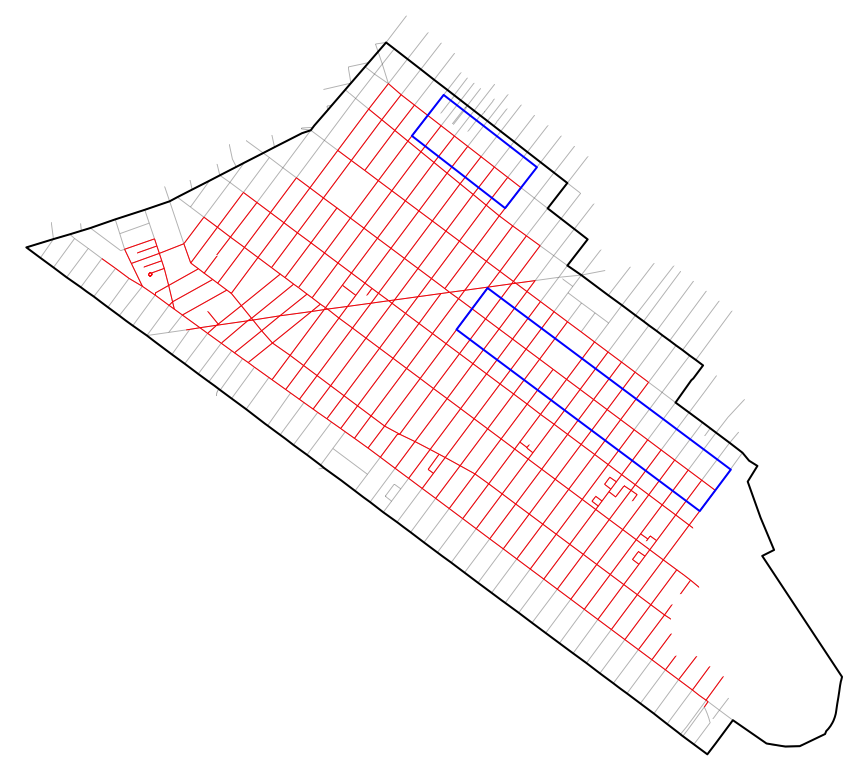
\includegraphics[scale=0.3]{plots/NullStreetExample83.png}
        \caption{The red streets in precinct 83 are ones that could potentially be used as null streets. The buffers (blue) are drawn around two potential null streets to illustrate how they meet the qualification for being completely contained in one precinct.}
    \label{fig:NullStreets}
\end{figure}
Assuming we can find a large number, $B$, of streets that are not near precinct boundaries, we can estimate a test statistic at each null street and use the distribution of these statistics as an estimate of $F_0$. Note that our procedure will be valid for any test statistic, though we will proceed with the estimate of $c$ from equation (\ref{eqn:TestStatistic}).  We denote these test statistics by $\widehat{\theta}^b$ for $b=1, \dots, B$.  We can then estimate the null distribution via $\widehat{F}_0(a) = \frac{1}{B} \sum_{b=1}^B I(\widehat{\theta}^b < a)$. For any $a$, we have that $\widehat{F}_0(a) \approx F_0(a)$ and we can construct rejection regions for our test using the relevant quantiles of the estimated null distribution. The intuition behind using this test to provide more robust hypothesis testing is that if assumption 1 does not hold at the boundary of interest, then it likely does not hold in other areas of New York City as well. For instance, there could be substantial spatial variability in individuals across New York City that changes far more locally than distances of $\delta$. We would not be able to account for this with observed covariates that are only available at the census-tract level, which is not sufficiently spatially resolved. However, it is likely that this variability is not unique to precinct boundaries, and that this variation also affects estimates at our resampled locations as well. By using these resampled locations, we are no longer relying on assumption 1 holding. To formalize our modified assumption, we first define $$d_1 = \Lambda_1(R_{\delta, 1}) - \Lambda_1(R_{\delta, 0}), \quad d_0 = \Lambda_0(R_{\delta, 1}) - \Lambda_0(R_{\delta, 0}),$$ 
where $d_1$ and $d_0$ capture the degree of the violation of assumption 1. Assumption 1 states that $d_1 = d_0 = 0$, which is a restrictive assumption in many settings. Letting $d_1^b$ and $d_2^b$ be the corresponding quantities at a resampled location, we can state the following assumption: \\
\\
\textbf{Assumption 1b:} When the null hypothesis is true, if $d_1,d_2 \sim G$ for some distribution $G$, then $d_1^b, d_2^b \sim G$. \\
\\
This assumption no longer makes the restrictive assumption that $d_1 = d_2 =0$, but rather assumes that these differences come from an unknown distribution, and that this distribution is the same as at the resampled locations. If this assumption holds and the null streets have similar levels of violations of assumption 1, then the test statistics found at the null streets should approximate the true null distribution $F_0$ and our resampling procedure will lead to valid inference. 

\subsection{Theoretical Implications (emmett)}
\label{sec:theory}
\textcolor{red}{add the maths involved using same notation as before}

\subsection{Global test of variation by precinct}
\label{sec:Global}

So far we have focused on performing a hypothesis test at a border between precincts A and B, however, there are many such borders in New York City. While there is interest in knowing whether any two bordering precincts have differential arresting practices, of arguably more interest is whether there is any variation across New York City in police precincts. In this setting we might wish to test whether the arrest rates differ by any precinct in New York City. It is difficult to compare any two precincts that are not bordering each other as we would not be able to focus on the regions of these two precincts that are geographically close. For this reason we restrict our attention to assessing whether any bordering precincts have differential precinct practices, which amounts to testing the following hypotheses:
\begin{align*}
    & H_0: \theta_{\delta, m} = 0 \text{ for } m=1, \dots, M \\
    & H_a: \theta_{\delta, m} \neq 0 \text{ for at least one } m.
\end{align*}
To perform this hypothesis test, we use a test statistic given by $\widehat{T} = \underset{m}{\text{max}} |\widehat{\theta}_{\delta, m}|$, which is analogous to using a minimum p-value over all hypothesis tests \citep{tippett1931methods}. Larger values of this test statistic provide additional evidence against the null hypothesis. We can use the same resampling procedure described above in order to perform inference using this test statistic. We approximate the distribution of $\widehat{T}$ under the null hypothesis using the empirical distribution of $\widehat{T}^b$ for $b=1, \dots, B$, where $\widehat{T}^b = \underset{m}{\text{max}} |\widehat{\theta}_{\delta, m}^b|$. 

\section{Simulation study (emmett)}
In order to confirm that the methods described above will allow for correct inference, a simulation study is performed by simulating the point process data on the New York City landscape. The simulation study will involve three ``classes'' of surfaces: (1) \textit{Hot Spots}, (2) \textit{Uniform}, (3) \textit{Random}. Heat maps of the surfaces are shown in Figure \textcolor{red}{(draw the picture)}  where the dark purple areas represent more arrests, and the light areas represent little to no crime. Regardless of the surface, our methodology should be robust to whatever biases are present in the point process data simulated.\\
\textcolor{red}{describe how the surface is made}\\
\textcolor{red}{describe how the "counts" are determined by sampling from a poisson process}\\

% Possible simulation studies:

% \begin{enumerate}
%     \item Set $\lambda(s) = c$ so that it is flat everywhere
%     \item Assume that  $\lambda(s)$ follows a Gaussian process with matern (or exponential) covariance matrix and vary the smoothness parameter. Inference should get worse as we decrease the amount of smoothness
%     \item Assume the surface is flat but has hotspots that are located randomly throughout the city that can mess up inference
% \end{enumerate}



\section{Analysis of precinct by precinct arrest rates}

Here we analyze the NYC arrest data to estimate the degree of variation in policing across the city as well as whether or not there are significant differences between individual precincts with regards to their arresting practices. We first provide our strategy for finding null streets in NYC and then highlight the impact that our procedure has on testing the null hypothesis of no treatment effects in NYC. Lastly, we apply our procedure to an analysis of 311 call data, which is known to not be related to policing precincts, to see if our procedure can correctly identify a null association in a situation where no treatment effect exists. 

\subsection{Finding null streets}
\label{sec:MatchesNYC}

%we were able to plot and count the number of arrests within a window length of any size on any street in NYC. With this ability, we can select streets that are completely contained in certain precincts, draw buffers around the streets and perform the ARIMA test on each street so that every street in NYC can have an associated p-value that can then be used to find the empirical distribution of each of the 164 observed p-values for the precinct borders. Now that we have the motivation, here was the exact process.

%While the CSCL data set was very large and housed a lot of information regarding each street in NYC, we needed more streets, and more variety in streets, in order to accurately obtain an empirical distribution as we described earlier. To begin, the dataset considered each block a separate street. In other words, say we have $5^{th}$ Ave. in NYC which is a long street that goes North-South. Along the way, it intersects with other streets going East-West. Instead of the dataset storing the entire $5^{th}$ Ave., it breaks it up into block-by-block pieces. This becomes an issue for our methodology later on because we want to find streets that resemble one of the 164 borders of interest, all of which span across multiple blocks. Hence, we needed to develop an algorithm that would combine streets in the CSCL data to create streets that more resemble the borders of interest. Using recursion, we did just that. The algorithm would select a street, find any streets near by that touched it, combine with those streets, then repeat the process until there were no more neighboring streets. Now the data set had streets that more resembled what we would find in our borders of interest. 

%From here, we could break down the larger streets as needed and could create this large new set of available streets to use. This also allowed us to filter for streets that were within a specific window length of the border (like the red streets in Figure \ref{fig:NullStreets}) in order to ensure that when we ran the ARIMA test, all of the arrests in the specific window would be from the same precinct, thus meeting our null conditions.

%Everything described above is cleaning and enhancing the data to then allow us to perform analysis. Now that we have this ``bank'' of streets to use for all buffer widths of interest, we can now begin obtaining the empirical distribution for the original p-values from the 164 precinct borders. If we fix a buffer width to look at, there is a list of streets available for use. Then, we choose a precinct buffer with an associated p-value whose distribution we wish to determine. In order to understand the empirical distribution, we need to pick, from that ``bank'' of null streets, which ones are similar to the border of interest. This similarity qualification is determined by the amount of crime that occurred in the same buffer. A null street is considered a ``match'' if

We obtained \textit{all} streets in NYC using the New York City Street Centerline (CSCL) data set, which contains over 100,000 streets in the city. This data provides information about each individual block in NYC, but does not provide information about full length streets that are comprised of multiple connected blocks. Therefore we first aggregated the blocks into full length streets, which could be used as potential null streets. It is important that we obtain a large number of null streets in order to obtain an accurate estimate of the null distribution of our test statistic. Many streets available in NYC are long avenues that are much longer than any of the precinct boundaries of interest, so we created additional streets by breaking long streets into smaller street subsections that can be used as null streets as well. Note that the number of streets available to us as null streets decreases as we increase the size of the buffer around the boundary, denoted by $\delta$. This is because a null street is only useful to us as long as it is more than $\delta$ away from any precinct boundary, thereby guaranteeing there is no effect of police precinct at that street. 

Now that we have a ``bank" of streets to use for any given buffer width $\delta$, we can proceed with finding good null streets for each precinct border. We want to find null streets that are as similar as possible to the precinct border they are being used to approximate under the null hypothesis as this makes assumption 1b more plausible. For this reason, we aim to find null streets that have similar levels of crime to the border of interest. To accomplish this, we randomly draw null streets for a particular precinct border that either 1) have total crime over the period of interest that is within 10\% of the total crime for that border, or 2) have a total number of crimes that is within 50 of the total number of crimes at the border of interest. We choose to identify null streets in this way to ensure that the null streets are similar to the border they are approximating, while also ensuring that we have enough null streets to approximate the null distribution of our test statistic. In a few instances, this algorithm led to less than 1000 null streets, and therefore we loosened the restrictions for these borders on what is considered a valid null street by taking the closest 1000 streets in terms of total crime to the border of interest. 

\subsection{Individual boundary estimates of precinct effects}

Now that we have constructed null streets for each of the 158 precinct boundaries, we can obtain corrected p-values for each boundary to perform a hypothesis test of whether there is a causal effect of police precinct near the boundary between the two precincts. The number of arrests in a particular region is intrinsically linked to the number of crimes in that region. For this reason, we first divide the number of arrests on either side of a boundary by the number of crimes in the corresponding region. This means that the $Z_t$ statistic used in our analyses is now the difference in arrest rates on the two sides of the boundary instead of the raw difference in arrest counts, though all other ideas apply directly. Figure \ref{fig:adjustedPval} shows the results of these analyses both before and after the correction using the null streets. The left panel shows the percentage of the 158 precinct boundaries for which the hypothesis test of no precinct effect was rejected both with and without our proposed correction. The uncorrected hypothesis tests show a large portion of significant differences with anywhere between 60\% and 70\% of the tests being rejected. Using the corrected approach, this number is far smaller, and very close to the type I error rate of 0.05. It is slightly above 0.05 for most buffer sizes $\delta$, and we will evaluate in Section \ref{sec:GlobalNYC} whether there is an overall effect of police precincts on arrest rates in NYC. The right panel of Figure \ref{fig:adjustedPval} shows the p-value histogram across the 158 hypothesis tests being evaluated for a buffer width of 500 feet. We see that this histogram looks quite close to uniformly distributed, which is in stark contrast to Figure \ref{fig:NaivePvalue}, which showed the corresponding distribution of uncorrected p-values. The large difference in results between the two approaches highlights that assumption 1 likely does not hold in this data set, but the more realistic assumption provided in assumption 1b is giving far more reasonable results. The results now indicate that while there could potentially be an effect of police precincts on arrest rates, this effect is very small and not widespread throughout the city. 

\begin{figure}[h]
    \centering
        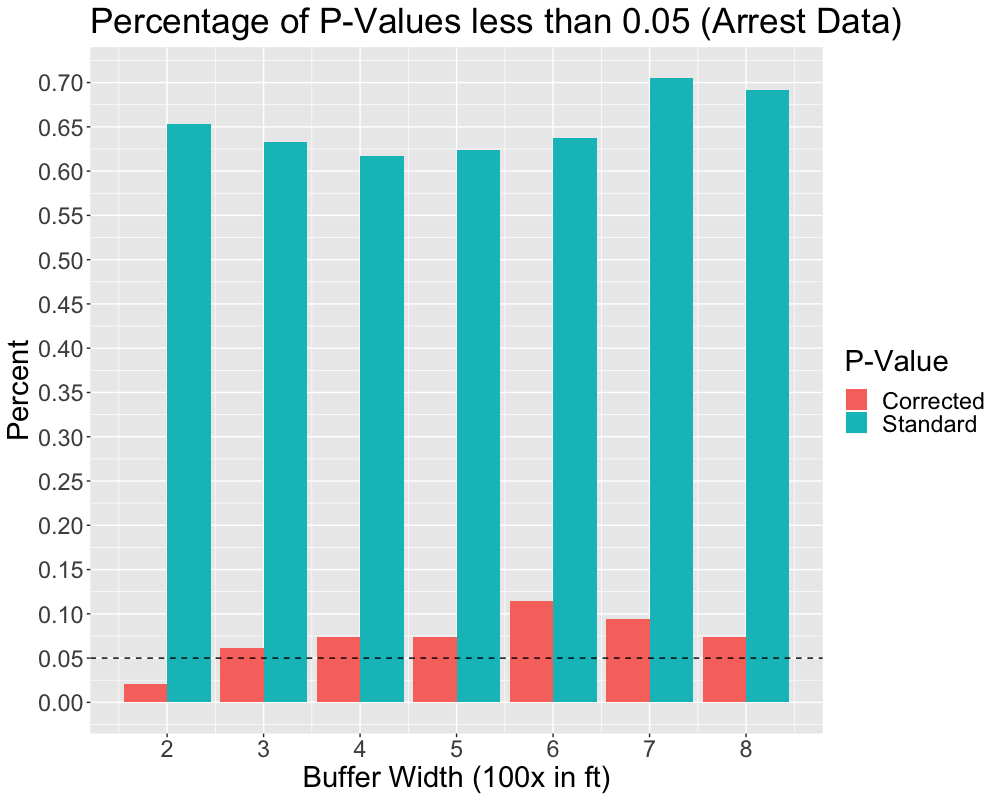
\includegraphics[width=0.45\linewidth]{plots/NewMatchesRejections.png}
    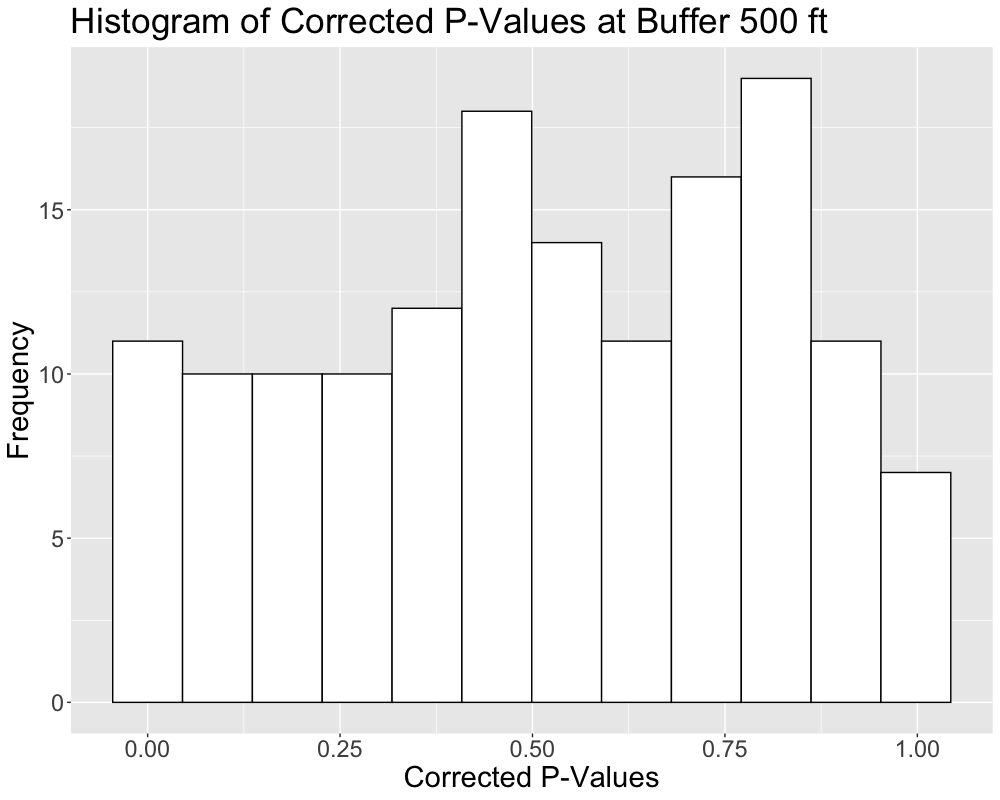
\includegraphics[width=0.45\linewidth]{plots/HistAdjPVal500.png}
        \caption{The left panel shows the percentage of p-values that are less than 0.05 before and after the correction as a function of buffer width. The right panel shows a histogram of the 158 corrected p-values at a buffer width of 500 feet.}
    \label{fig:adjustedPval}
\end{figure}

\subsection{Global variation in arrest rates}
\label{sec:GlobalNYC}

In this section, we apply the approach of Section \ref{sec:Global} to assess whether there is any effect of police precincts on arrest rates in NYC. We first calculate the test statistic $\widehat{T} = \underset{m}{\text{max}} |\widehat{\theta}_{\delta, m}|$ at the precinct borders to assess the magnitude of the overall precinct effect across the entire city. To understand the distribution of this test statistic under the null hypothesis of no precinct effect, we also calculate this test statistic using null streets to obtain $\hat{T}^b = \underset{m}{\text{max}} |\widehat{\theta}_{\delta, m}^b|$ for $b=1, \dots, B$, using the matches discussed in Section \ref{sec:MatchesNYC}. We perform this procedure $B=5000$ times for each of the 7 distinct buffer sizes $\delta$ that we consider. The results of this procedure can be seen in Figure \ref{fig:GlobalObsPval}. We see that the p-value is small for buffer widths of 200 and 300 feet, and then becomes larger (around 0.5) for the remaining buffer widths considered. Regardless of the buffer width, the largest test statistic for the true precinct boundaries is found at the boundary between precincts 40 and 42. For small buffer widths this association leads to statistical significance at the 0.05 level. As can be seen in the right panel of Figure \ref{fig:GlobalObsPval}, when the buffer is increased, the null distribution of the maximum test statistic shifts to the right. This is likely due to increasing violations of assumption 1, which becomes less plausible as we increase $\delta$. This shift increases the cutoff value for a test statistic to be deemed significant, which leads to larger p-values for our hypothesis test. 
\begin{figure}[h]
    \centering
        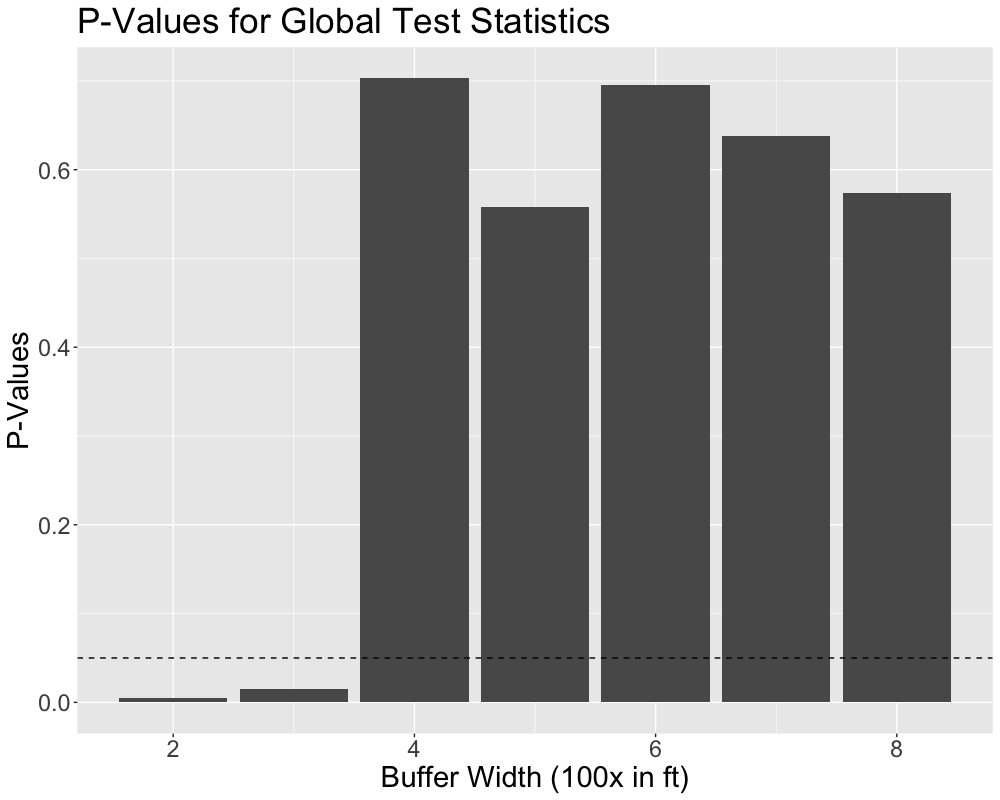
\includegraphics[height=0.35\linewidth]{plots/GlobalTestMax.png}         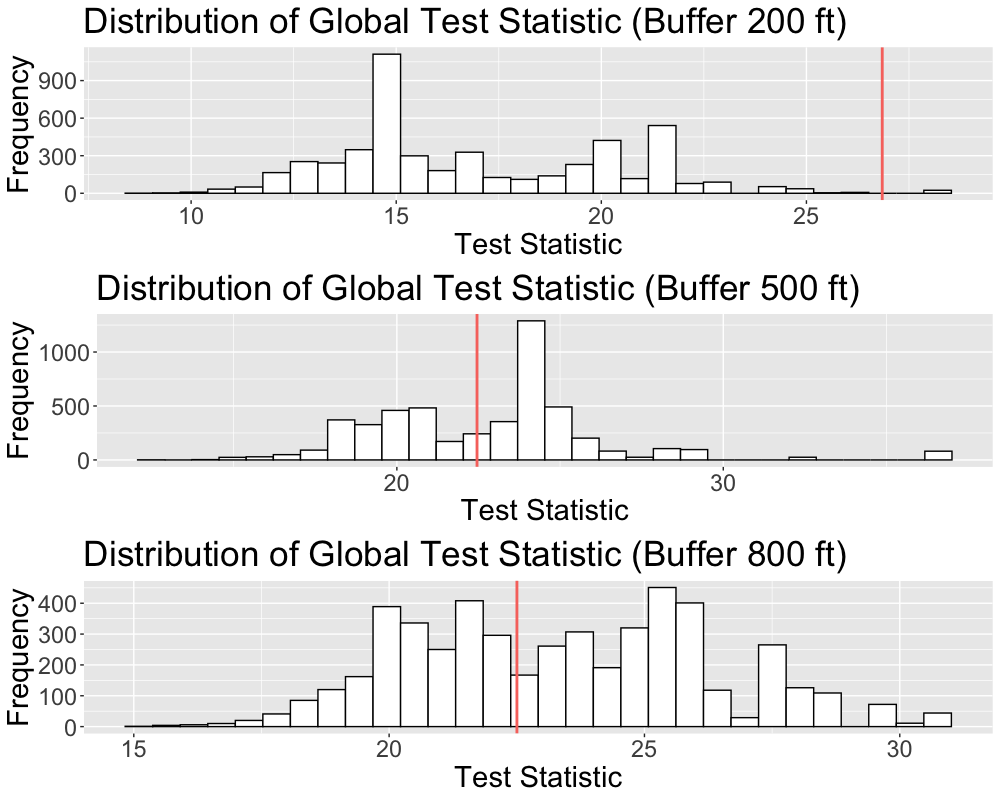
\includegraphics[height=0.35\linewidth]{plots/DistributionGlobalTestStat.png}
        \caption{Results from the global test of variation in policing across NYC. The left panel shows the p-value as a function of the buffer width. The right panel shows the histogram of resampled test statistics from our proposed procedure for three different buffer widths. The vertical line corresponds to the observed test statistic at the true precinct borders.}
    \label{fig:GlobalObsPval}
\end{figure}

\subsection{Negative control analysis}

In order to verify the validity of our methodology, we applied our procedure to an outcome that is believed to have no association with police precincts. This outcome data comes from all 311 Service Request Calls from 2010 to 2020 in NYC. This data set is similar to the the primary data set on arrest locations as it contains specific spatial locations for each 311 call as well as where the call was directed. The data was filtered to exclude calls directed to the NYPD in order to further separate the data from any possible association to police precincts. We define $Y_{\delta, a}$ and $Y_{\delta, b}$ to be the total number of 311 calls made within a distance of $\delta$ from the border between precincts A and B that fall in either precinct A or B, respectively. Under the null hypothesis of no precinct effect on 311 calls we know that 
$$Y_{\delta, a} \sim \text{Binomial}(Y_{\delta, a} + Y_{\delta, b}, 0.5).$$
Using this distributional result, we can perform a hypothesis test to evaluate the null hypothesis of no precinct effect at the border between precincts A and B. This will only lead to a valid hypothesis test if assumption 1 holds for the new outcome. If it does not, we would expect the p-value distribution to be shifted to the left and the percentage of rejected tests to be well above the desired 0.05 level. In that case we would like to see if our proposed inferential procedure based on assumption 1b works in obtaining the correct type I error rates.

Figure \ref{fig:NegControlRej} illustrates the percent of significant associations estimated out of the 158 borders both before and after the proposed correction. Without the correction, the percentage of rejected tests is far above the desired 0.05 level as we see anywhere from 50\% to 75\% rejection rates, with an increasing trend as a function of the buffer width. Given that this outcome is thought to have no association with police precincts, these results point to a lack of validity of the statistical test being run. After the correction, the results drop to a far more reasonable level with roughly 5\% rejections for buffer widths between 200 and 500 feet. For buffer widths between 600 and 800 feet the percentage of rejections increases to around 10\%, though this is still a substantial improvement on the uncorrected hypothesis tests. Overall, the negative control analysis provides further justification for using our proposed procedure, and gives increased belief in our findings on arrest rates in the previous sections.

\begin{figure}
    \centering
    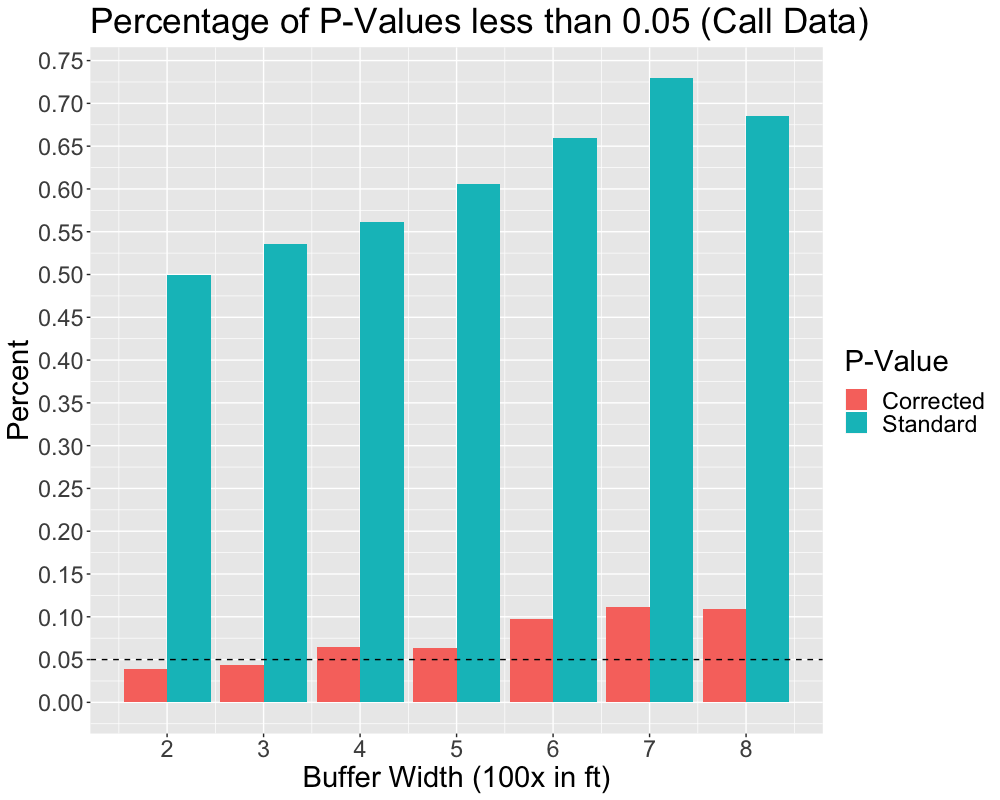
\includegraphics[scale=0.25]{plots/NegControlFinal.png}
        \caption{The number of p-values that are less than 0.05 before and after correction using our methodology on the negative control data.}
    \label{fig:NegControlRej}
\end{figure}



\section{Discussion}

In this manuscript we have proposed an approach to geographic regression discontinuity designs that weakens the local randomization assumption that is typically made in such studies. By leveraging the rich spatio-temporal information in our data on crime and arrests in NYC, we showed that valid hypothesis tests can be re-constructed even in the presence of certain violations of local randomization assumptions around the boundary of interest. The main idea is to find new boundaries that behave similarly to the boundary of interest, but do not live near the border of two police precincts and therefore necessarily have no precinct effect. In the analysis of NYC arrest data we found that analyses relying on local randomization assumptions lead to very strong conclusions that police precincts greatly impact police rates, while our approach based on resampling new streets leads to the conclusion that there is little to no effect of police precincts on arresting practices. 

Our procedure was shown to work in a geographic regression discontinuity setting, though it is potentially applicable to other settings as well. The only requirement is that new cutoffs of the running or forcing variable must be used where no treatment effect exists, and that the data set is rich enough to provide a large number of these new locations that are sufficiently separated from each other. While our procedure is able to provide statistical validity (type I error control) to tests of the hypothesis of no treatment effect, it is not able to correct for biases in estimation and provide consistent estimates of treatment effects themselves. Further research is required to reduce the assumptions needed for estimation of treatment effects in regression discontinuity designs.

\bibliographystyle{authordate1}
\bibliography{References}

\end{document}



